\documentclass[a4paper,12pt]{article}

\usepackage[T2A]{fontenc} 
\usepackage[utf8]{inputenc}
\usepackage[english,russian]{babel}
\usepackage{listings}
\usepackage[dvips]{graphicx}
\usepackage{indentfirst}
\usepackage{color}
\usepackage{hyperref}
\usepackage{amsmath}
\usepackage{amssymb}
\usepackage{geometry}
\geometry{left=1.5cm}
\geometry{right=1.5cm}
\geometry{top=2cm}
\geometry{bottom=2cm}

\graphicspath{{images/}}

\begin{document}
\sloppy

\lstset{
	basicstyle=\small,
	stringstyle=\ttfamily,
	showstringspaces=false,
	columns=fixed,
	breaklines=true,
	numbers=right,
	numberstyle=\tiny
}

\newtheorem{Def}{Определение}[section]
\newtheorem{Th}{Теорема}
\newtheorem{Lem}[Th]{Лемма}
\newenvironment{Proof}
	{\par\noindent{\bf Доказательство.}}
	{\hfill$\scriptstyle\blacksquare$}
\newenvironment{Solution}
	{\par\noindent{\bf Решение.}}
	{\hfill$\scriptstyle\blacksquare$}


\begin{flushright}
	Кринкин М. Ю. группа 504 (SE)
\end{flushright}

\section{Домашнее задание 1. Вариант 001111}

\begin{figure}[h]
	\noindent\center{
		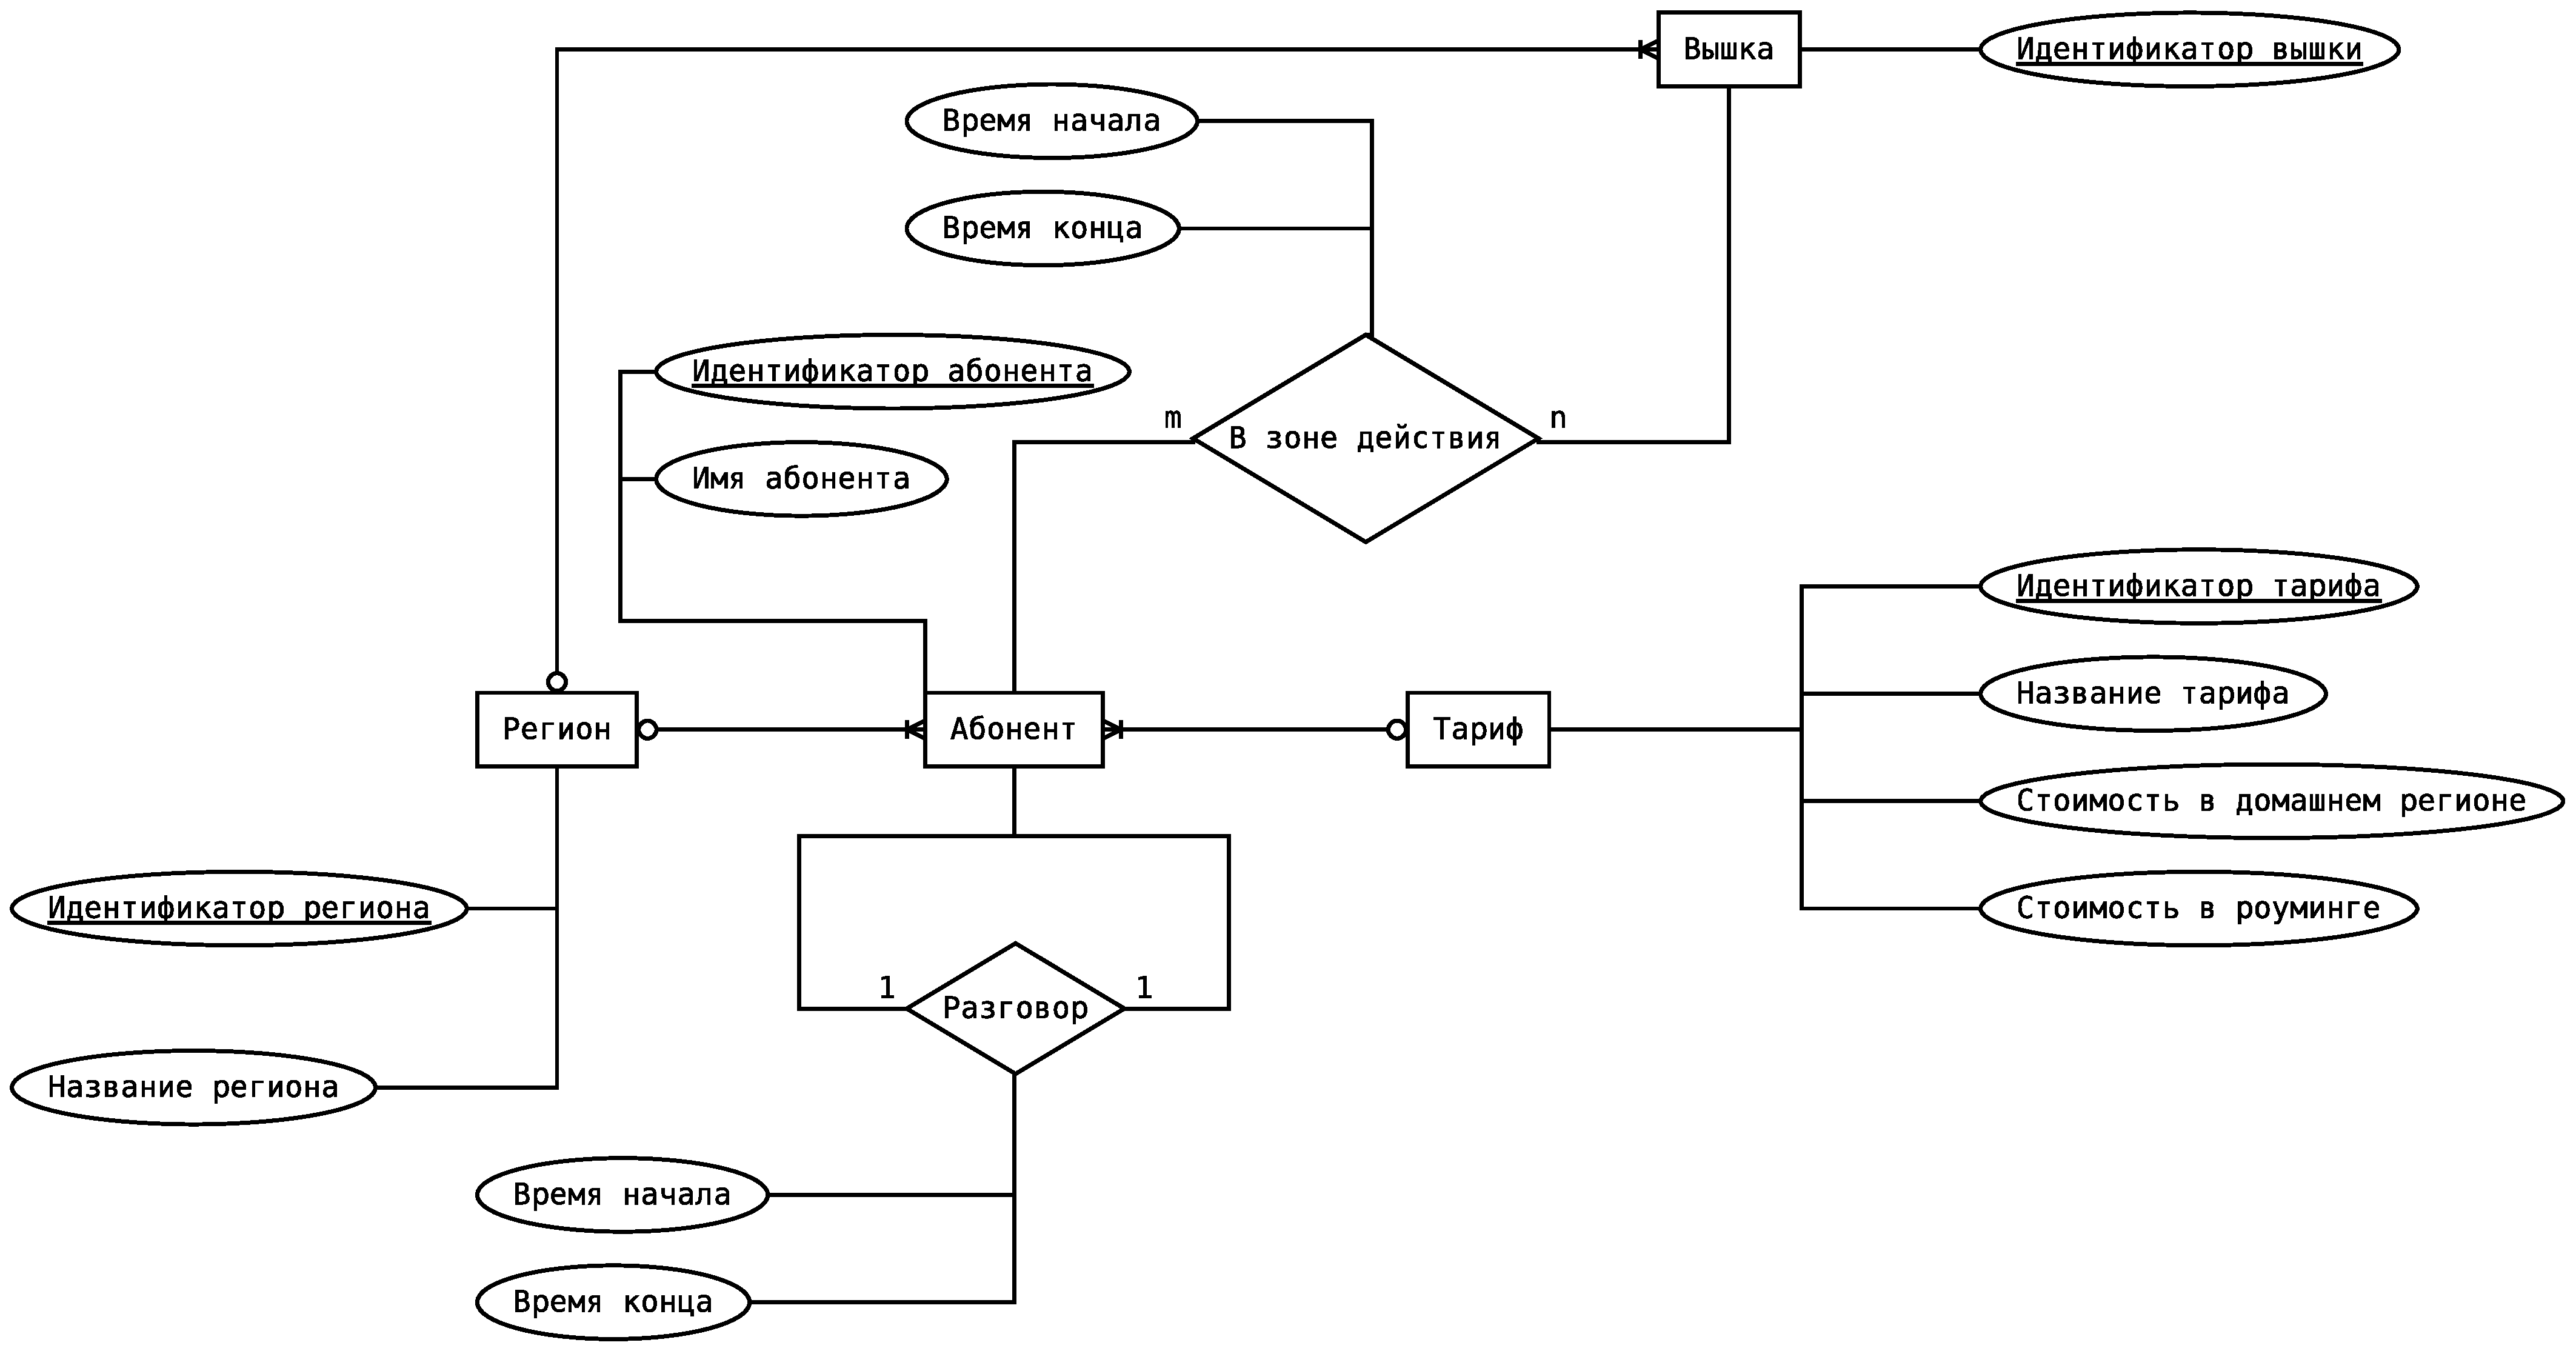
\includegraphics[width=0.9\linewidth]{er_diag}
	}
	\caption{ER-диаграмма базы данных сотового оператора Флатлайн}
	\label{pic::er_diag}
\end{figure}

\paragraph{Дать определение следующим терминам:}
\begin{enumerate}
\item \underline{Хранимое определение базы данных.} Как я понимаю, хранимое определение базы данных - внутренняя схема (определение структуры хранения) базы данных, в которой определяются типы хранимых записей, существующие индексы, способы представления хранимых полей, физическая упорядоченномть хранимых записей. Внутренняя схема соответствует 3 (самому нижнему) уровню модели ANSI/SPARC. При этом внутренняя схема не определяет физическое представление базы данных (например в виде дорожек на диске и т. п.), так как за это отвечает ОС. (Вольный пересказ К. Дейта).

\item \underline{Распределенная обработка.} Распределенная обработка предплагает наличие некоторого числа компьютерных систем, которые связаны коммуникационной сетью таким способом, чтобы определенная задача обработки данных могла быть распределена между этими системами в сети. При этом, если мы говорим о базах данных, то доступ к распределенной базе данных должен быть для пользователя прозрачным - распределенность никак не должна влиять на взаимодействие пользователя с базой, т. е. должна быть скрыта от него. Распределенные базы данных, скорее всего, имеют свои специфические свойства, связанные с необходимостью синхронизации данных на разных машинах, распределением нагрузки и тд.

\item \underline{Логический проект базы данных.} Логический проект (или концептуальный) базы данных - логическая структура предназначенная для хранения некоторого массива данных. Эта логическая структура должна включать опредление значимых сущностей и их атрибутов, а также определять связи сущностей между собой и ограничения накладываемые на атрибуты. В идеале логическое проектирование это самостоятельная стадия, которая не должна зависеть от физической реализации проекта, но на практике это не всегда так. Из методов логического проектирования баз данных мне изестны ER-метод и метод универсального отношения (последний мало распространен и подходит, наверно, только для проектирования маленьких баз данных).
\end{enumerate}

\begin{figure}[h]
	\noindent\center{
		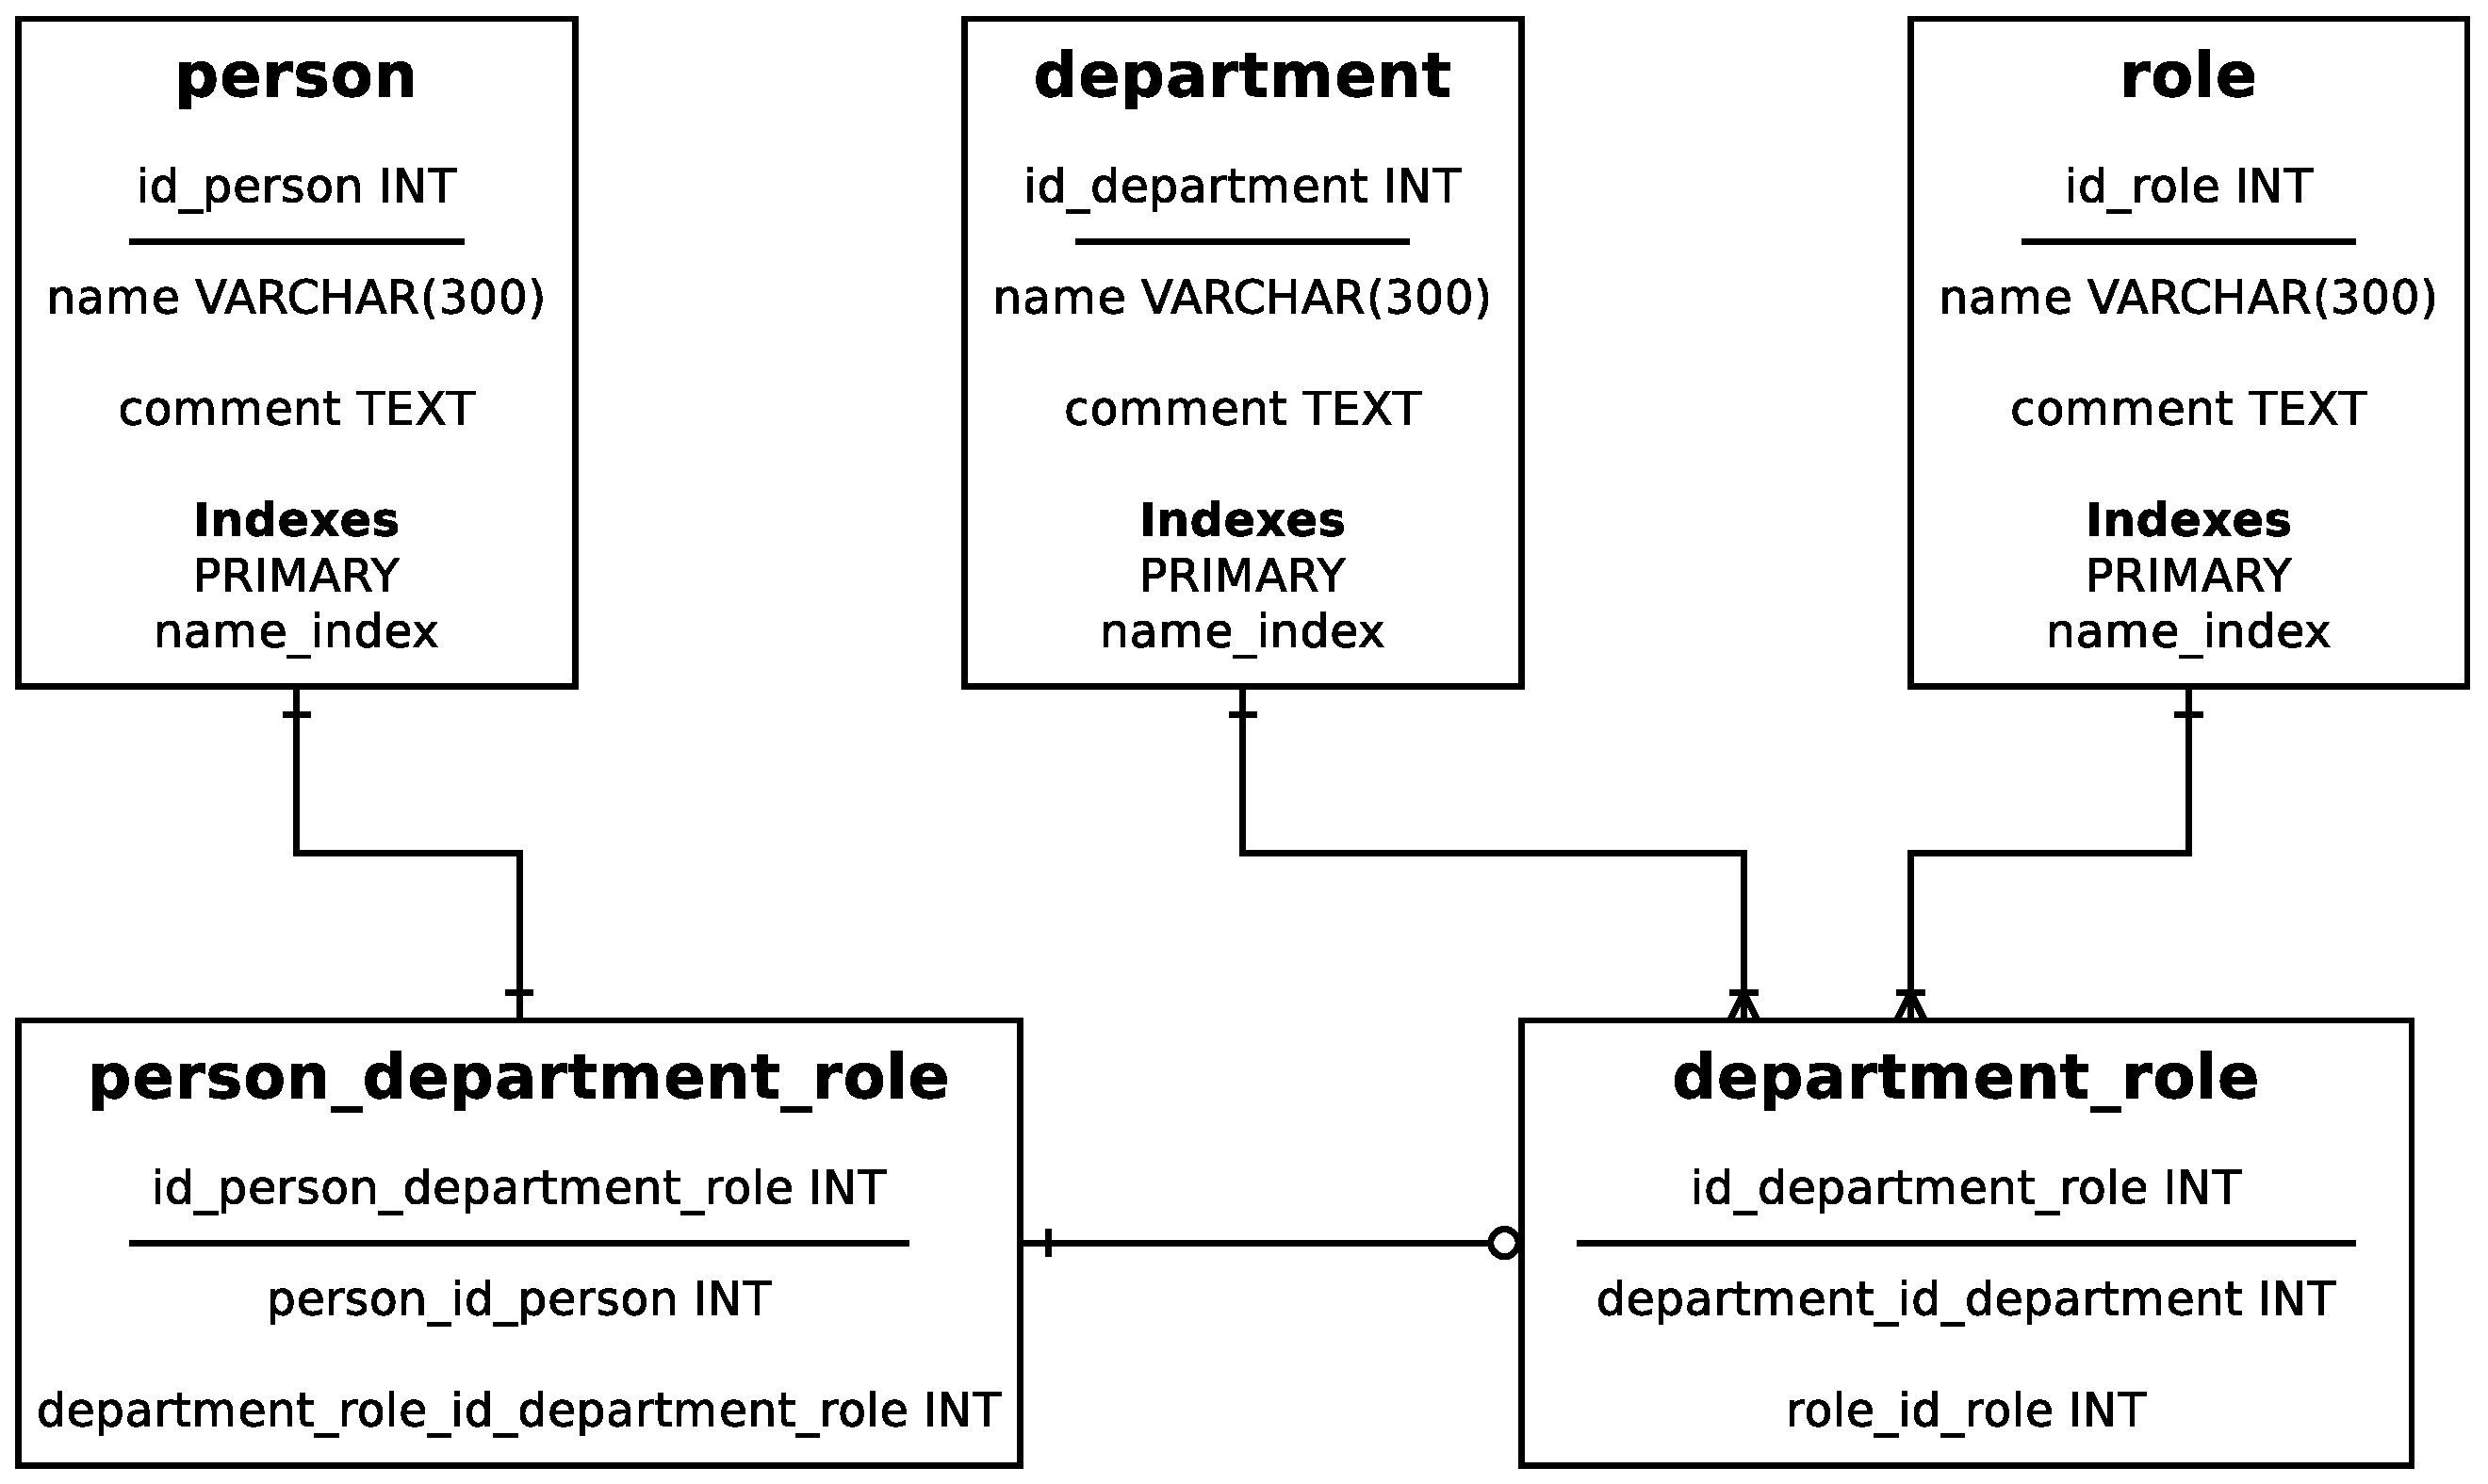
\includegraphics[width=0.9\linewidth]{schema}
	}
	\caption{Определить предметную область}
	\label{pic::schema}
\end{figure}

Судя по названиям, это описание базы данных некторого отдела кадров (хотя для полноты картины не хватает зарплаты). В организации есть некоторое количество отделов и несколько видов должностей (видно из названий отношений). Каждому отделу требуются определенные должности (отношение department role), каждый человек (person) занимет некоторую должность, примем, что один человек может занимать только одну должность, и обратно одну должность может занимать только один человек, при этом возможна ситуация, что какая-либо должность оказалась незанятой (допустим, не успели подобрать человека на эту должность), в этом случае связь между person department role и department role со стороны последнего не обязательна. Также, допустим, что нам не нужна информация о людях, которые не занимают никаких должностей, тогда связь между person и person department role один к одному и обязательна с обоих сторон. Каждому отделу может соотетствовать несколько должностей, кроме того одна и та же должность может присутствовать сразу в нескольких отделах, то есть связь department с deaprtment role один ко многим, и аналогичная связь role с department role.

\end{document}
